\section{Special Functions}
\subsection{Integral Functions}
\subsubsection{Gamma Function, $\Gammaa{x}$}
Defined by the integral:
\begin{equation}
    \Gammaa{x}=\intt{0}{\infty}t^{x-1}\e{-t}dt,\quad\text{ convergent for }x>0
\end{equation}
\subsubsection*{Properties:}
\begin{center}
    \nicerbox{0.8}{
    \begin{enumerate}
        \item Recurrence relation:\vspace{0.5ex}\\
        $\displaystyle\Gammaa{x+1}=x\Gammaa{x},\quad\text{where }x=1,2,3,\ldots$
        \item In general:\vspace{0.5ex}\\
        $\displaystyle\Gammaa{x+1}=x!\Gammaa{1}=x!,\quad\text{where }\Gammaa{1}=1$
        \item Reverse recurrence relation:\vspace{0.5ex}\\
        $\displaystyle\Gammaa{x}=\frac{\Gammaa{x+1}}{x}$
        \item Negative values of $x$:
        \begin{enumerate}[a.]
            \item Integers:
            $\displaystyle\Gammaa{0}=\infty;\quad\Gammaa{-x}=\pm\infty$
            \item Fraction ($x=\frac{n}{2}$):
            $\displaystyle\Gammaa{-x}=\frac{\Gammaa{-x+1}}{-x}$
        \end{enumerate}
        \item Duplication formula:\vspace{0.5ex}\\
        $\Gammaa{n+\frac{1}{2}}=\displaystyle\frac{\Gammaa{2n}\sqrt{\pi}}{2^{2n-1}\Gammaa{n}}$
        \item $\Gammaa{\frac{1}{2}}=\sqrt{\pi}=\displaystyle2\intt{0}{\infty}\e{-u^2}du$
        \item[i.] Stirling formula:\vspace{0.5ex}\\
        $\displaystyle n!\approx \sqrt{2\pi n}\ n^n\e{-n},\quad\text{where $n$ is large}$
        \item[ii.] $\displaystyle\intt{0}{\infty}x^n\cdot\e{-ax}dx=\frac{\Gammaa{n+1}}{a^{n+1}}=\frac{n!}{a^{n+1}}$
        \item[iii.] $\displaystyle\intt{0}{\infty}\e{-ax^2}dx=\frac{1}{2}\sqrt{\frac{\pi}{a}}$
        \item[iv.] $\displaystyle\intt{0}{\infty}x^m\cdot\e{-ax^2}dx=\frac{\Gammaa{\frac{m+1}{2}}}{2a^{\bracket{m+1}/2}}$
    \end{enumerate}
    }
\end{center}
\newpage
\begin{figure}[!ht]
    \centering
    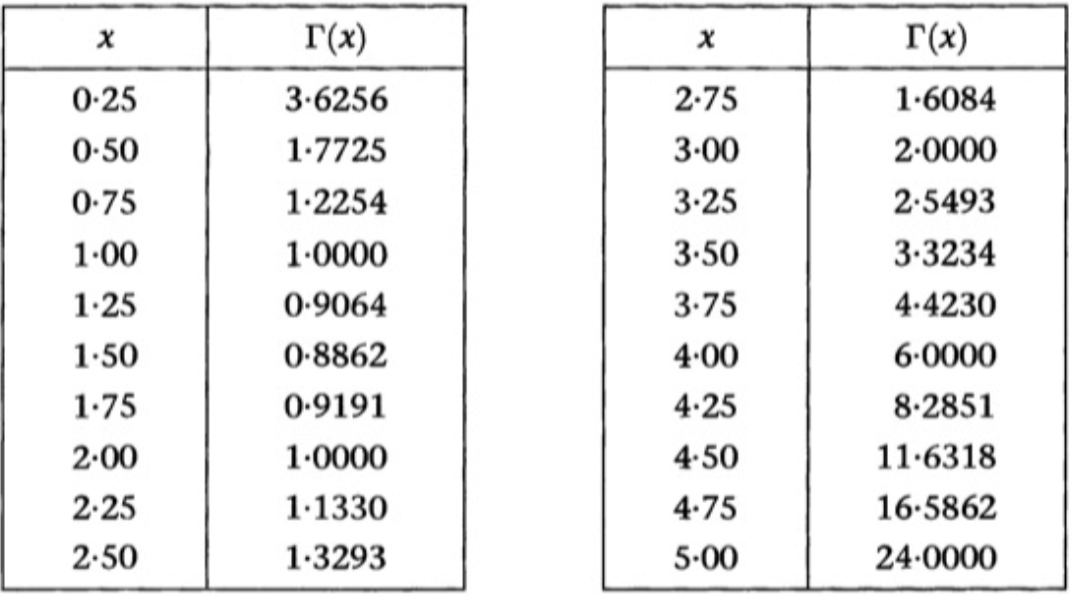
\includegraphics[width=0.7\textwidth]{Images/3.1.png}
    \caption{Table of values of $\Gammaa{x}$}
    \label{fig:3.1}
\end{figure}
\begin{figure}[!ht]
    \centering
    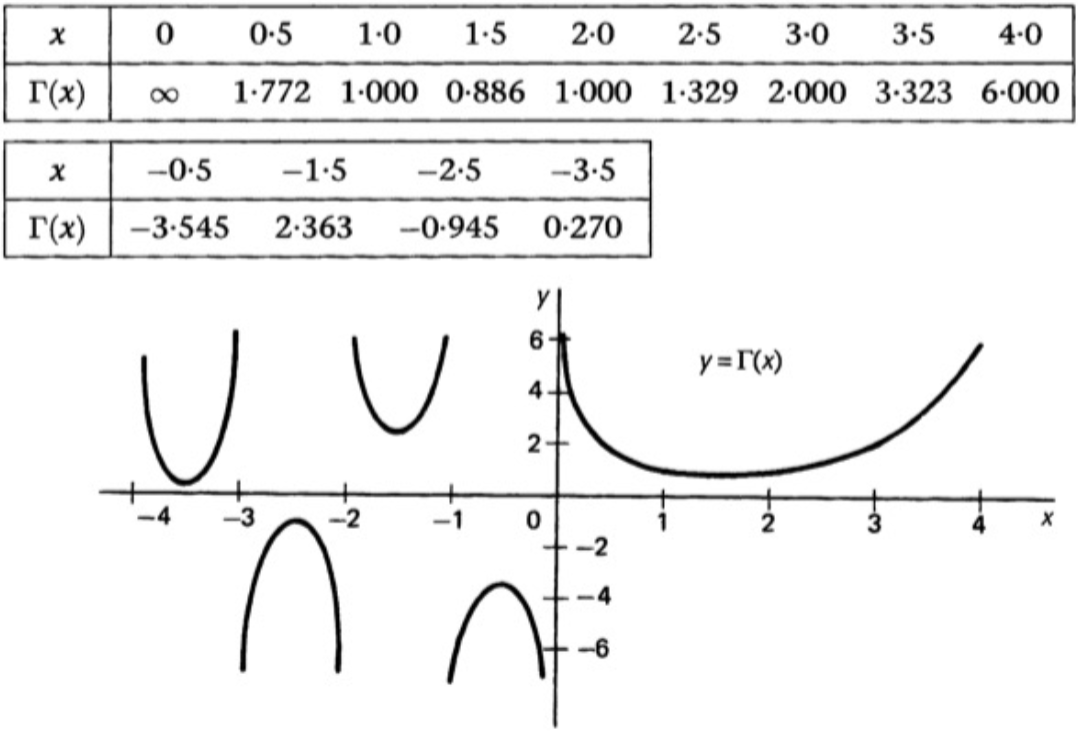
\includegraphics[width=0.7\textwidth]{Images/3.2.png}
    \caption{Values and plot of $y=\Gammaa{x}$}
    \label{fig:3.2}
\end{figure}
\newpage
\subsubsection{Beta Function, $\Beta{m,n}$}
Defined by the integral:
\begin{equation}
    \Beta{m,n}=\intt{0}{1}x^{m-1}\bracket{1-x}^{n-1}dx,\quad\text{convergent for }m,n>0
\end{equation}
\subsubsection*{Properties:}
\begin{center}
    \nicerbox{0.8}{
    \begin{enumerate}
        \item Symmetry property:\vspace{0.5ex}\\
        $\Beta{m,n}=\Beta{n,m}$
        \item Trigonometric form:\vspace{0.5ex}\\
        $\displaystyle\Beta{m,n}=2\intt{0}{\pi/2}\sinnN{2m-1}{\theta}\cossN{2m-1}{\theta}d\theta,\quad\bracket{\text{sub }x=\sin^2\theta}$
        \item Reduction formula:\vspace{0.5ex}\\
        $\displaystyle\Beta{m,n}=\frac{\bracket{m-1}\bracket{n-1}}{\bracket{m+n-1}\bracket{m+n-2}}\Beta{m-1,n-1}$
        \item In general:\vspace{0.5ex}\\
        $\displaystyle\Beta{m,n}=\frac{\bracket{m-1}!\bracket{n-1}!}{\bracket{m+n-1}!}$
        \item $\displaystyle\Beta{k,1}=\Beta{1,k}=\frac{1}{k}$
        \item $\Beta{\frac{1}{2},\frac{1}{2}}=\pi$
    \end{enumerate}
    }
\end{center}
\subsubsection{Relation between Gamma and Beta Functions}
\begin{equation}
    \Beta{m,n}=\Beta{m,n}=\frac{\bracket{m-1}!\bracket{n-1}!}{\bracket{m+n-1}!}=\frac{\Gammaa{m}\Gammaa{n}}{\Gammaa{m+n}},\quad m,n\in\mathbb{R}
\end{equation}
\subsubsection*{Reduction Formula of Sines and Cosines}
\begin{enumerate}
    \item $\displaystyle\intt{0}{\pi/2}\sin^n\bracket{x}dx=\frac{n-1}{n}\intt{0}{\pi/2}\sin^{n-2}\bracket{x}dx,\quad S_n=\frac{n-1}{n}S_{n-2}$
    \item $\displaystyle\intt{0}{\pi/2}\cos^n\bracket{x}dx=\frac{n-1}{n}\intt{0}{\pi/2}\cos^{n-2}\bracket{x}dx,\quad C_n=\frac{n-1}{n}C_{n-2}$
    \item $\displaystyle\intt{0}{\pi/2}\sinnN{m}{x}\cossN{n}{x}=\frac{m-1}{m+n}\intt{0}{\pi/2}\sinnN{m-2}{x}\cossN{n}{x}dx\equiv I_{m,n}=\frac{m-1}{m+n}I_{m-2,\ n}$
    \item $\displaystyle\intt{0}{\pi/2}\sinnN{m}{x}\cossN{n}{x}=\frac{n-1}{m+n}\intt{0}{\pi/2}\sinnN{m}{x}\cossN{n-2}{x}dx\equiv I_{m,n}=\frac{n-1}{m+n}I_{m,\ n-2}$
\end{enumerate}
\subsection{Error Function}
Defined as:
\begin{equation}
    \erff{x}=\frac{2}{\sqrt{\pi}}\intt{0}{x}\e{-t^2}dt
\end{equation}
From the definition of $\Gammaa{\frac{1}{2}}$, we can find the limits:
\begin{equation}
    \lim\limits_{x\to\infty}\sbracket{\erff{x}}=\frac{2}{\sqrt{\pi}}\intt{0}{\infty}\e{-t^2}dt=\frac{1}{\sqrt{2}}\cdot\Gammaa{\tfrac{1}{2}}=1
\end{equation}
Representing the exponential function in the integral with Maclaurin series:
\begin{equation}
    \erff{x}=\frac{2}{\sqrt{\pi}}\summation{n=0}{\infty}\frac{\bracket{-1}^nx^{2n+1}}{n!\bracket{2n+1}}
\end{equation} 
Consequently, $\erff{x}$ is an odd function:
\begin{equation}
    \erff{-x}=-\erff{x}
\end{equation}
\begin{figure}[!ht]
    \centering
    \begin{tikzpicture}
    \begin{axis}[xlabel=$x$,ylabel=$erf(x)$,title= {Error function in pgfplots $erf(x)=\frac{2}{\sqrt{\pi}}\int_{0}^{x}e^{-t^{2}}\, dt$},legend style={draw=none},legend pos=south east,grid=major,enlargelimits=false]
    \addplot [domain=-3:3,samples=50,red,no markers] gnuplot[id=erf]{erf(x)};
    % Note: \addplot function { gnuplot code } is alias for \addplot gnuplot { gnuplot code };
    \addplot [domain=-3:3,samples=2,black,no markers] gnuplot[id=x-axis]{0};
    \addplot [domain=-0.01:0.01,samples=2,black,no markers] gnuplot[id=y-axis]{150*x};
    \addplot [domain=-3:3,samples=2,cyan,no markers,dotted,thick] gnuplot[id=a1]{1};
    \addplot [domain=-3:3,samples=2,cyan,no markers,dotted,thick] gnuplot[id=a2]{-1};
    \legend{$\erff{x}$}
    \end{axis}
    \end{tikzpicture}
    \caption{Plot of error function $\erff{x}$}
    \label{fig:3.3}
\end{figure}
\subsubsection{Complementary Error Function, $\erfcc{x}$}
Defined as:
\begin{equation}
    \erfcc{x}=\frac{2}{\sqrt{\pi}}\intt{x}{\infty}\e{-t^2}dt
\end{equation}
which is related to the Error function by relation:
\begin{equation}
    \erfcc{x}=1-\erff{x}
\end{equation}
\subsubsection{Relationship between Error and Gaussian Function}
Gaussian integral is defined as:
\begin{equation}
    \Phi\bracket{x}=\frac{1}{\sqrt{2\pi}}\intt{-\infty}{x}\e{-t^2/2}dt,\quad\text{where}\quad\Phi\bracket{x}=\frac{1}{\sqrt{2\pi}}\intt{-\infty}{\infty}\e{-t^2/2}dt=1
\end{equation}
For positive $x$. $\Phi\bracket{x}$ is related to $\erff{x}$ by:
\begin{equation}
    \Phi\bracket{x}=\frac{1}{2}+\frac{1}{2}\erff{\frac{x}{\sqrt{2}}}
\end{equation}
\subsection{Elliptic Functions}
\nicerbox{1}{\centering An \textit{integral is elliptic} if the \textit{\textbf{integrand is a rational function of $x$ and $\mathbf{\sqrt{P\bracket{x}}}$}}.\\(where $P\bracket{x}$ is a polynomial of degree $3$ or $4$)
\begin{equation}
    \intt{0}{1}\frac{dx}{\sqrt{\bracket{1-2x^2}\bracket{4-3x^2}}}
\end{equation}}
\subsubsection{Standard and Alternative Form of Elliptic Function}
\subsubsection*{i) Of the First Kind}
\begin{equation}\label{eqn:3.13}
    \FF{k,\phi}=\intt{0}{\phi}\frac{d\theta}{\sqrt{1-k^2\sinnN{2}{\theta}}}\quad\text{or}\quad F\bracket{k,x}=\intt{0}{x}\frac{dt}{\sqrt{\bracket{1-t^2}\bracket{1-k^2t^2}}}
\end{equation}
\begin{center}
    where $0<k<1$ and ($0\leq\phi\leq\frac{\pi}{2}$ or $0\leq x\leq 1$)
\end{center}
\subsubsection*{ii) Of the Second Kind}
\begin{equation}\label{eqn:3.14}
    E\bracket{k,\phi}=\intt{0}{\phi}\sqrt{1-k^2\sinnN{2}{\theta}}\ d\theta\quad\text{or}\quad E\bracket{k,x}=\intt{0}{x}\sqrt{\frac{1-k^2u^2}{1-u^2}}du
\end{equation}
\begin{center}
    where $0<k<1$ and ($0\leq\phi\leq\frac{\pi}{2}$ or $0\leq x\leq 1$)
\end{center}
\subsubsection{Complete Elliptic Functions}
\nicerbox{1}{\centering For Equations (\ref{eqn:3.13}) and (\ref{eqn:3.14}): \textit{If} $\mathit{\phi=\frac{\pi}{2}}$, the \textbf{\textit{integral is said to be complete}.} Then:
\begin{align}
    F\bracket{k,\tfrac{\pi}{2}} \text{ denoted by }F\bracket{k}\quad&\text{and}\quad E\bracket{k,\tfrac{\pi}{2}} \text{ denoted by }E\bracket{k}\\
    \FF{k}=\intt{0}{\frac{\pi}{2}}\frac{d\theta}{\sqrt{1-k^2\sinnN{2}{\theta}}}\quad&\text{and}\quad E\bracket{k}=\intt{0}{\frac{\pi}{2}}\sqrt{1-k^2\sinnN{2}{\theta}d\theta}\nonumber
\end{align}}
\subsubsection{Useful Techniques}
\subsubsection*{Situation 1}
For integrals of the form:
\begin{equation}
    I=\intt{0}{\frac{\pi}{2}}\frac{d\theta}{\sqrt{1+4\sin^2{\theta}}}
\end{equation}
Solve by letting $\theta=\frac{\pi}{2}-\psi\Rightarrow\sin\theta=\cos{\psi}$ and changing the limits. Then:
\begin{equation*}
    I=\intt{\frac{\pi}{2}}{0}\frac{-d\psi}{\sqrt{1+4\cos^2\psi}}=\intt{0}{\frac{\pi}{2}}\frac{d\psi}{\sqrt{1+4\sbracket{1-\sin^2\psi}}}=\intt{0}{\frac{\pi}{2}}\frac{d\psi}{\sqrt{5-4\sin^2\psi}}
\end{equation*}
\subsubsection*{Situation 2}
For integrals of the form:
\begin{equation}
    I=\intt{0}{2}\frac{dt}{\sqrt{\bracket{4-t^2}\bracket{9-t^2}}}
\end{equation}
Select denominator $\bracket{4-t^2}$. Then let $t=2\sin\theta\Rightarrow dt=2\cos\theta\ d\theta$ and changing the limits:
\begin{equation}
    I=\intt{0}{\frac{\pi}{2}}\frac{2\cos\theta \ d\theta}{\sqrt{\bracket{4-4\sin^2\theta}\bracket{9-4\sin^2\theta}}}=\intt{0}{\frac{\pi}{2}}\frac{2\cos\theta \ d\theta}{2\cos\theta\cdot\sqrt{9-4\sin^2\theta}}=\intt{0}{\frac{\pi}{2}}\frac{d\theta}{\sqrt{9-4\sin^2\theta}}\nonumber
\end{equation}